\section{Introduction}\label{section:Introduction}
The western part of the Eiffel region is known for strong volcanism is the past 50 million years \citep{NiklasPlumpe.2015}. This work focuses on the region close to the Rockeskyller Kopf as it differs from the surrounding volcanism. First huge sanidine crystals were found in the 1920s \citep{hopmann1914spuren} and studied since then. The mineralogic analysis indicate a phonolitic eruption close to a highly differentiated magma that is atypical for the study area \citep{MarcBoxberg.2011}. 

During a phonolitic eruption magmatic tuffs as well as fragments of the neighbouring host rock are emitted. Most of the erupted material is assumed to fall back into the crater and therefore we find highly fractured rocks and magmatic tuffs inside the diatreme structure \citep{white2011maar}. Due to surface erosion and deposition of new sediments the crater is buried under a new geologic layer and cannot necessarily be identified with geomorphologic analysis. Therefore non-intrusive geophysical methods have to be applied in order to reveal those structures. Finding and modelling the volcanic eruption center of this phonolitic eruption will help to improve the existing knowledge about the regional geology of the Westeiffel around the Rockeskyller Kopf. 

The first efforts to find the volcanic source of these crystals are documented in \citet{mertes1983aufbau}. He conducted a magnetic survey which indicates a strong anomaly. Several follow-up geophysical surveys using magnetics, seismic methods and electrical resistivity tomography (ERT) were conducted in order to find and model the volcanic structure in the subsurface (\cite{MarcBoxberg.2011,NiklasPlumpe.2015,NadineHauburg.2016,DanielSchneider.2017,TimGilberti.2020,HannahMues.2013}). First initial models are mainly based on the magnetic measurements, however, a more detailed model of the volcanic source is yet to be determined. 

Goal of the upcoming Master thesis is to obtain a more detailed subsurface model of the volcanic structure which is indicated by the strong magnetic anomaly which is described in \citet{mertes1983aufbau,MarcBoxberg.2011}. Using joint inversion approaches a geologic model of the volcanic diatreme based on several geophysical methods will be generated. To better understand the sensitivity of the different methods to a diatreme structure in the subsurface, this paper presents a synthetic data study of a representative diatreme structure as it could be found in the field. For model generation, forward calculations and data inversion the open-source library PyGIMLI \citep{Ruecker2017} is used. The synthetic data study includes the ERT method, traveltime tomography and gravimetric data. The synthetic data study will show which parts of the subsurface structure can be retrieved from the different geophysical methods.

The forward model used in this synthetic data study is designed to mimic a typical diatreme structure. To simplify the model generation and to speed up forward calculations and inversions, a 2D section through a simplified diatreme structure is considered. The forward model is based on \citet{white2011maar} as well as first subsurface models based on the geophysical surveys that were mentioned before. To consider a more realistic model the diatreme structure shows an irregular upper boundary and is hosted in a horizontally layered subsurface consisting of a shallow soil layer, two sandstone layers and the basement. The resulting 2D section is shown in \ref{figure:synthetic_model}.

\begin{figure}[H]
\centering
\noindent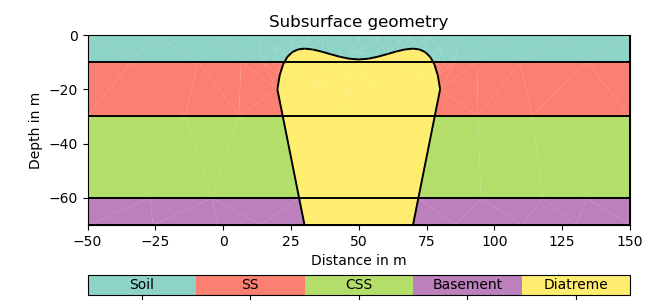
\includegraphics[width=0.8\textwidth]{Figures/Model.png}
\caption[Synthetic model of simplified diatreme structure]{Synthetic model of simplified diatreme structure. SS is referring to the first sandstone layer and CSS refers to a second, more consolidated sandstone layer.}
\label{figure:synthetic_model}
\end{figure}

\begin{figure}[H]
\centering
\noindent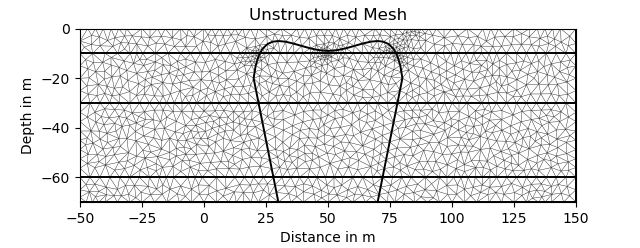
\includegraphics[width=0.8\textwidth]{Figures/Mesh.png}
\caption[Unstructired mesh]{Unstructured, triangular mesh used to discrtize the subsurface geometry.}
\label{figure:mesh}
\end{figure}

+++ Add subfigure also including mesh on right side